\documentclass[12pt,a4paper]{article}
\usepackage{algorithm, algpseudocode, amsmath, amssymb, amsthm, csquotes, empheq, geometry, graphicx, hyperref, listings, multirow, siunitx, subcaption, upgreek}
\usepackage[italicdiff]{physics}
\usepackage[section]{placeins}
\usepackage[justification=centering]{caption}

\title{Computational Physics\\Problem Set 10}
\author{Saleh Shamloo Ahmadi\\Student Number: 98100872}
\date{January 3, 2022}

\hypersetup{colorlinks=true, urlcolor=cyan}
\newcommand{\fig}{../fig}

\begin{document}
	\maketitle
	\section{System Configuration}
	All data is taken in a system with side length 30 in reduced units and 100 particles.

	\section{Trajectory}
	Animations for different phases and phase transition can be found under the \texttt{anim} directory.
	\texttt{gas.mp4}, \texttt{liquid.mp4}, and \texttt{solid.mp4} show the different phases and
	\texttt{phasechange.mp4} shows how the fluid undergoes a phase transition as the temperature is
	lowered.
	
	\newgeometry{top=0.7in, bottom=1in}
	\section{Equilibrium}
	\begin{figure}[htb!]
		\centering
		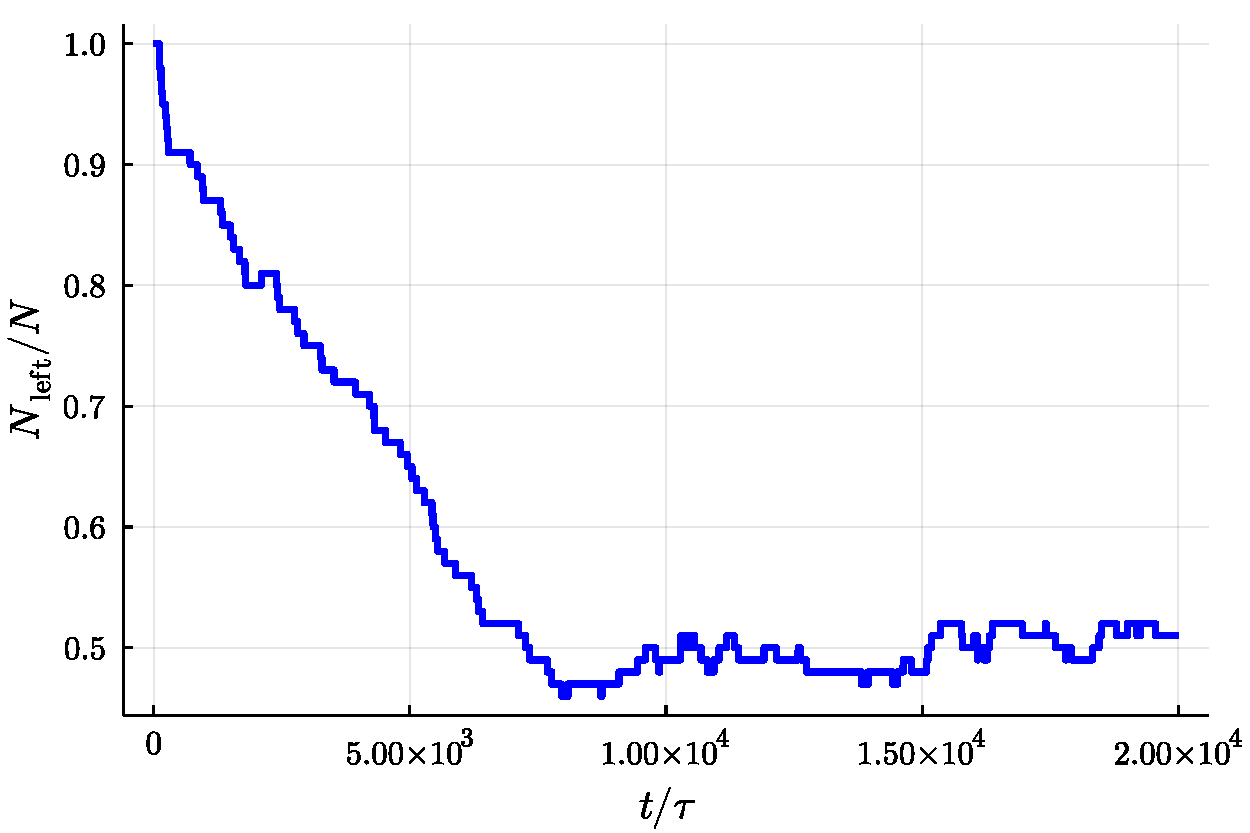
\includegraphics[width=\linewidth]{\fig/leftsidenum}
		\caption{The ratio of the particles on the left side of the container to the total number of particles
			starts out equal to 1.0 (the initial configuration is a simple cubic lattice on the left side of the
			container) and approaches 0.5 atequilibrium.}
	\end{figure}
	\begin{figure}[htb!]
		\centering
		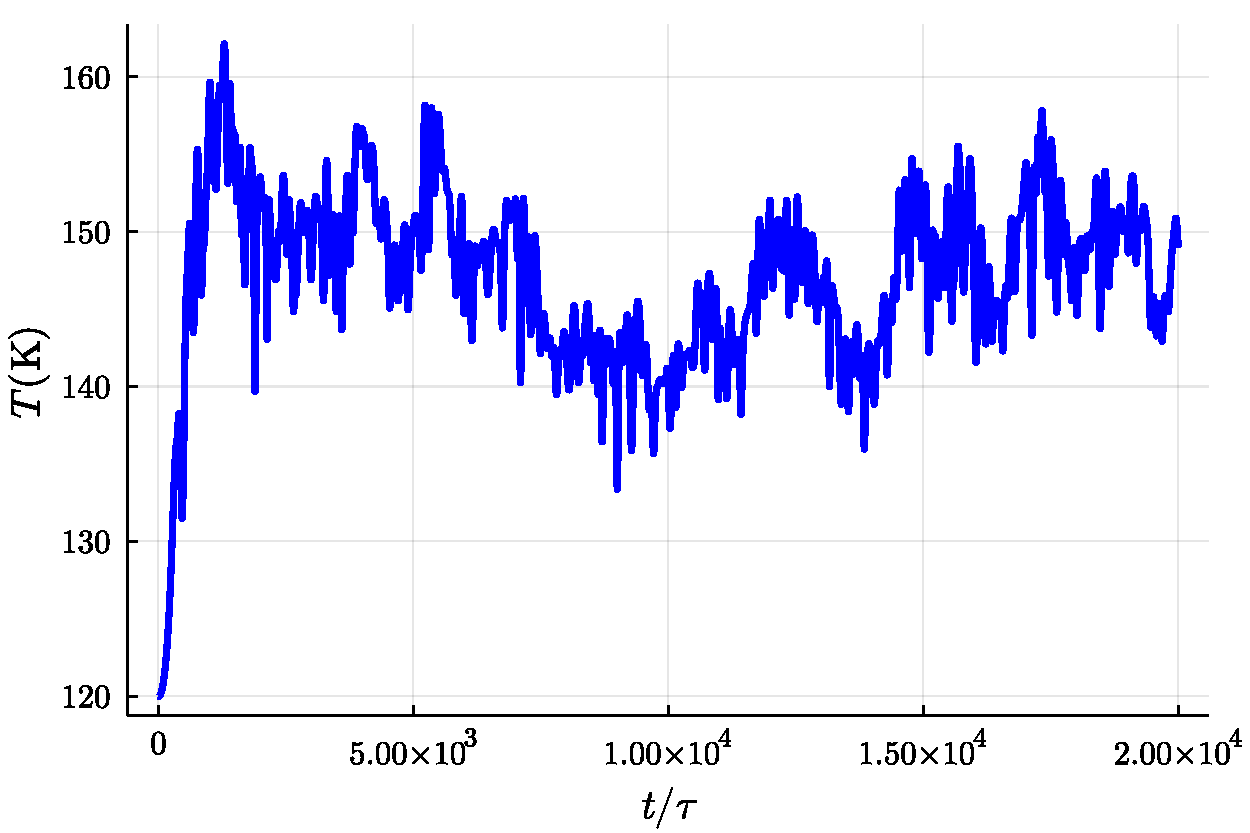
\includegraphics[width=\linewidth]{\fig/temperature}
		\caption{The temperature fluctuates around a roughly constant temperature as the system approaches equilibrium.}
	\end{figure}
	\begin{figure}[htb!]
		\centering
		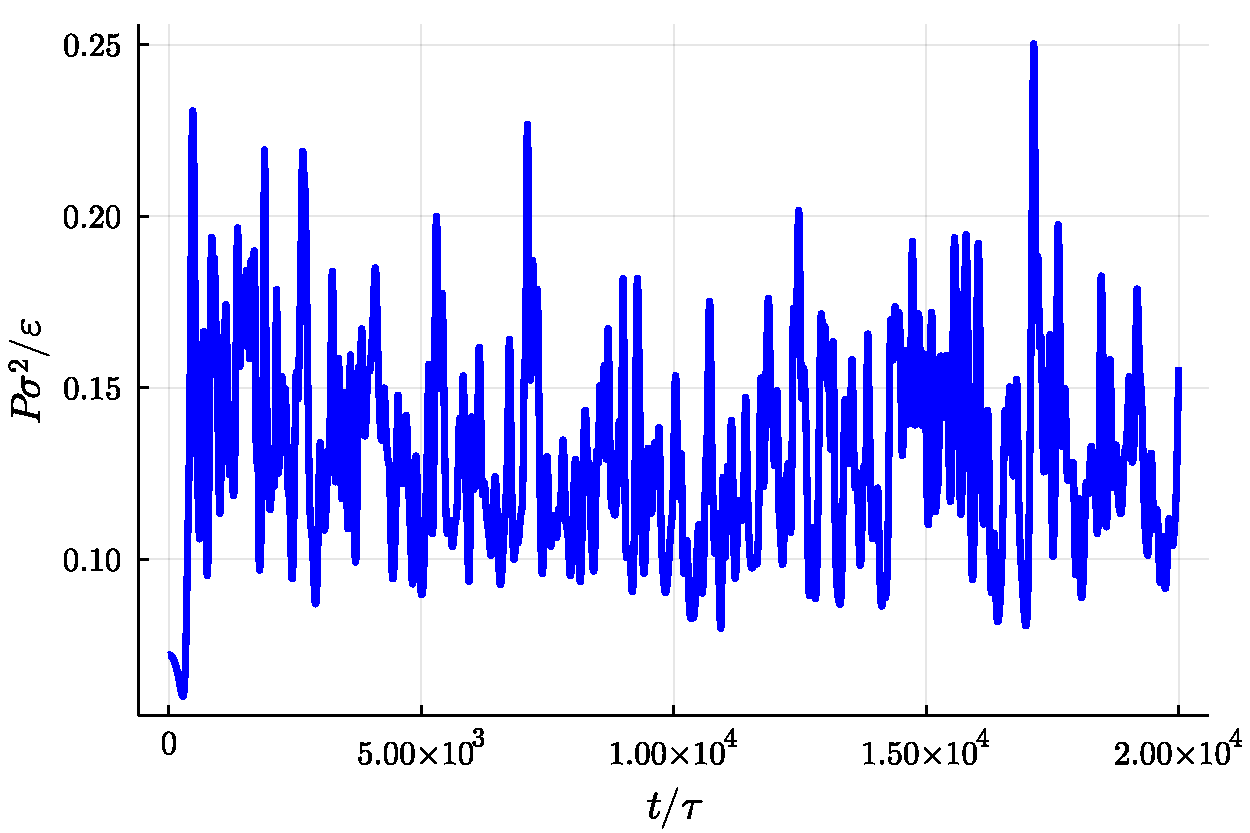
\includegraphics[width=\linewidth]{\fig/pressure}
		\caption{The pressure has a more chaotic behaviour.}
	\end{figure}
	\begin{figure}[htb!]
		\centering
		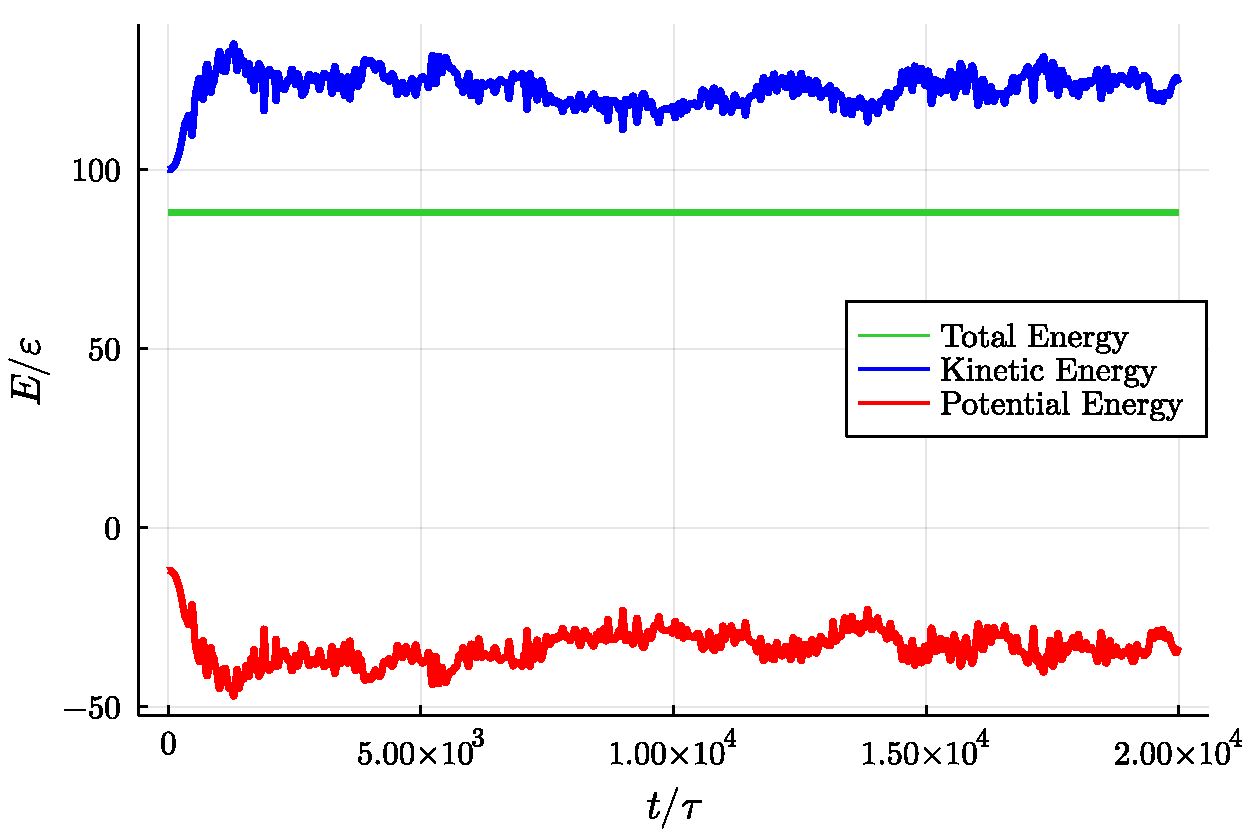
\includegraphics[width=\linewidth]{\fig/energy}
		\caption{The total energy stays constant, as you would expect.}
	\end{figure}
	\begin{figure}[htb!]
		\centering
		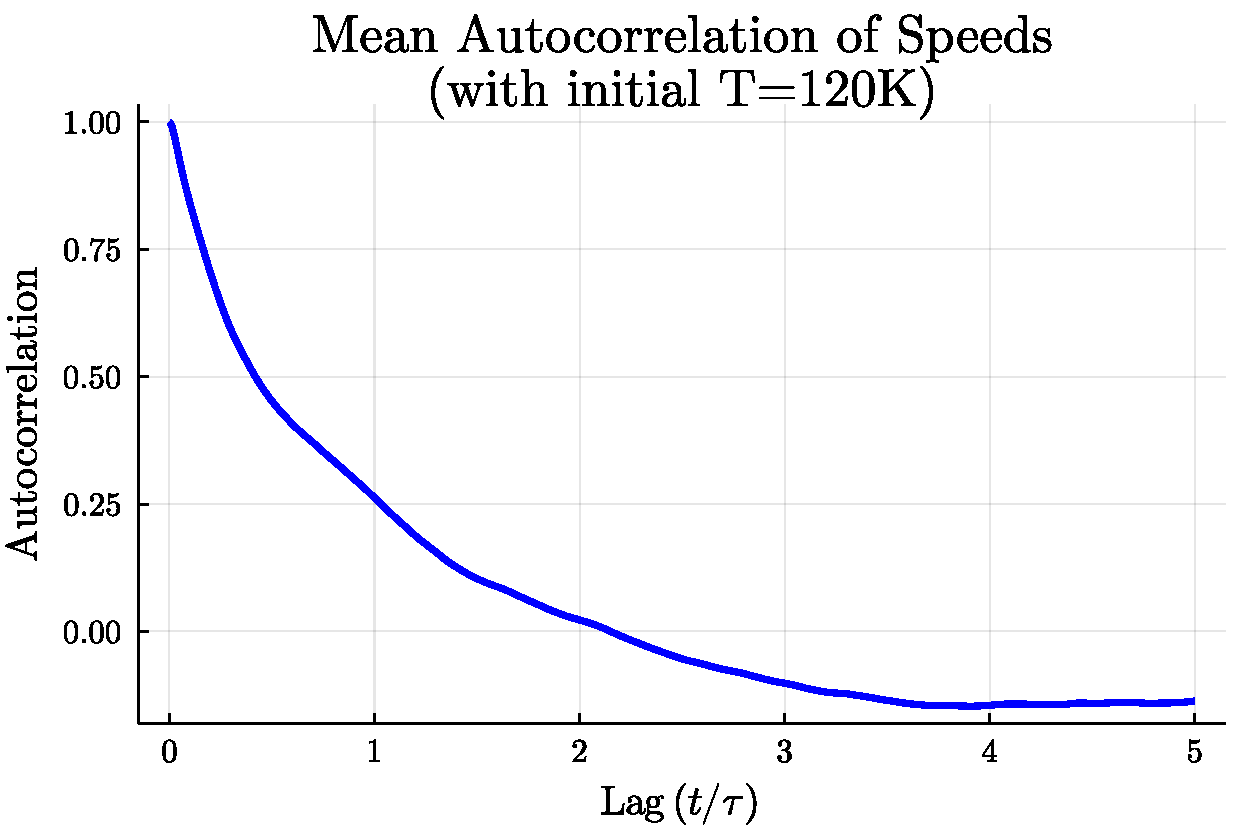
\includegraphics[width=\linewidth]{\fig/autocor}
		\caption{The relaxation time is $(0.782 \pm 0.008)\tau$ with the average temperature around 140 kelvin
			(if $C_v(t)$ is the autocorrelation of speed with time difference $t$, then $C_v(t)\sim e^{-t/\xi}$
			and the relaxation time is defined to be equal to $\xi$)}
	\end{figure}
	\section{Van der Waals Equation}
	The Van der Waals equation is
	\begin{equation}
		\qty(P + a\frac{n^2}{V^2})(V-nb) = nRT.
	\end{equation}
	Rearranging the terms to get the pressure $P$ in terms of $T$
	\begin{equation}
		P = \frac{nR}{V-nb}T - \frac{n^2}{V^2}a.
	\end{equation}
	In reduced units (we also set $N_A = 1$)
	\begin{equation}
		P = \frac{1}{V/N-b^*}T - \frac{N^2}{V^2}a^*.
	\end{equation}
	With the data I collected, simple linear regression gives 
	\begin{equation}
		P = (0.1310 \pm 0.0004)T - (0.028 \pm 0.001).
	\end{equation}
	Therefore
	\begin{empheq}[left=\empheqlbrace]{align}
		a^* &= 2.26 \pm 0.08 \\
		b^* &= 1.37 \pm 0.02
	\end{empheq}
	\begin{figure}[htb!]
		\centering
		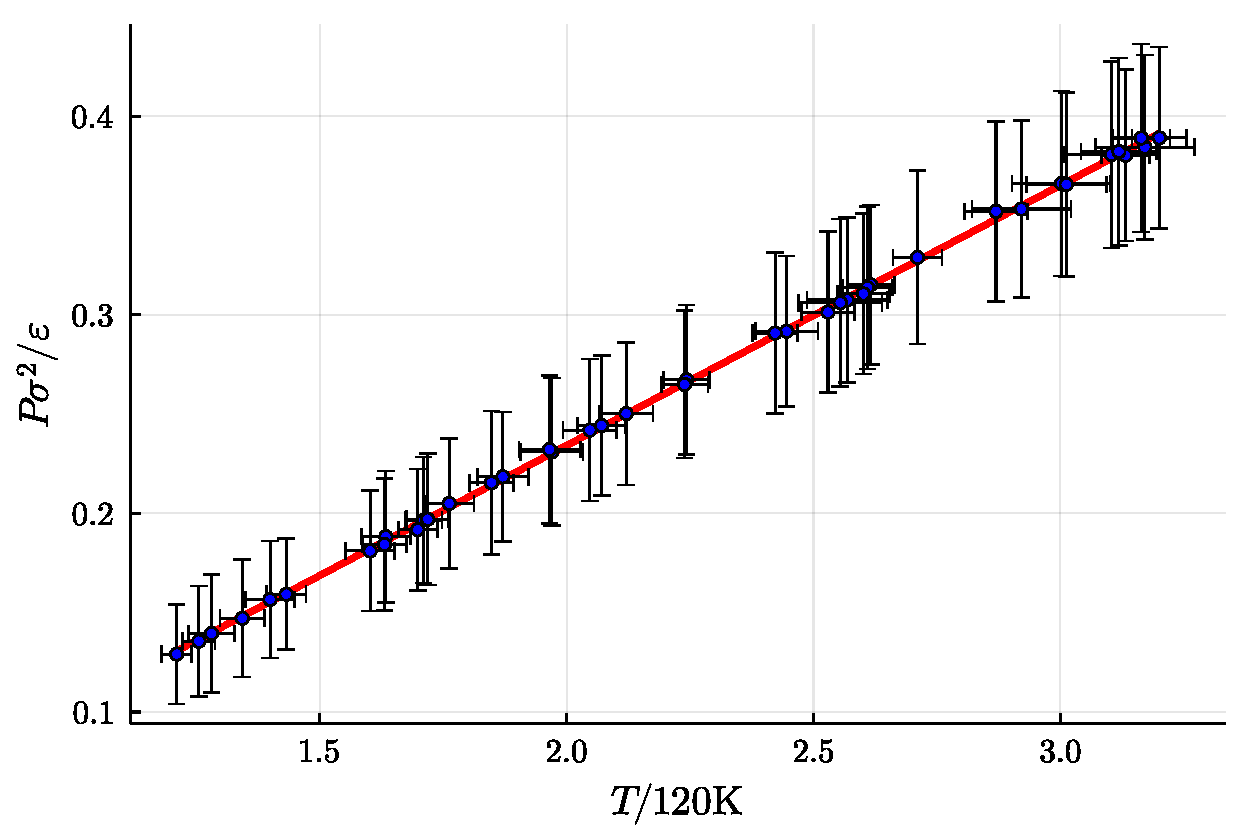
\includegraphics[width=\linewidth]{\fig/vanderwaals}
		\caption{$P-T$ plot for the mean pressures and temperatures at equilibrium and the fitted Van der Waals
			equation line. The exact equilibrium temperature is hard to control, so instead of equally distanced
			temperature, these points have equally distanced energies.}
	\end{figure}
\end{document}
